% What a TikZ picture or a formula may load. A package not loaded here is one a figure cannot use.
\documentclass[tikz,border=2pt]{standalone}
\usepackage{amsmath,amssymb,amsfonts,mathtools,bm}
\usepackage{xcolor}
\usepackage{pgfplots}
\pgfplotsset{compat=1.18}
\usetikzlibrary{arrows.meta,positioning,calc,shapes.geometric,shapes.misc,decorations.pathreplacing,decorations.markings,fit,backgrounds,patterns,matrix,chains,trees,automata,intersections,angles,quotes}
\usepgfplotslibrary{fillbetween}
\begin{document}
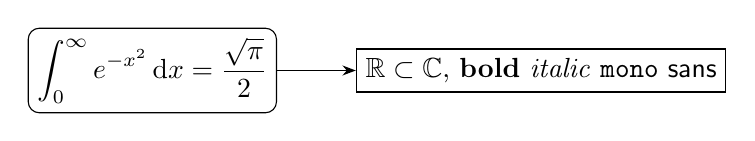
\begin{tikzpicture}
  \node[draw, rounded corners] (a) {$\displaystyle \int_0^\infty e^{-x^2}\,\mathrm{d}x = \frac{\sqrt{\pi}}{2}$};
  \node[draw, right=of a] (b) {$\mathbb{R} \subset \mathbb{C}$, \textbf{bold} \textit{italic} \texttt{mono} \textsf{sans}};
  \draw[-{Stealth}] (a) -- (b);
\end{tikzpicture}
\begin{tikzpicture}
  \begin{axis}[xlabel=$x$, ylabel=$y$, legend entries={$\sin x$}]
    \addplot[domain=0:6.28, samples=40] {sin(deg(x))};
  \end{axis}
\end{tikzpicture}
\end{document}
